\chapter{ELMy H-Modes on C-Mod}\label{ch:Elmy}

The ELMy H-mode \cite{Wagner1982,Keilhacker1984}, described in \cref{sec:hcr_elmy}, is the most commonly-accessed high-performance regime on major tokamak experiments.  The bursty transport driven by ELMs provides sufficient relaxation of the particle confinement in H-mode to allow stationary operation without excessive impurity accumulation; as such, the ELMy H-mode is considered the baseline operating regime for ITER \cite{ITER1999,Shimada2007}.  However, on ITER-scale devices the pulsed heat loading associated with ELMs drives unacceptable levels of erosion and damage to plasma-facing wall and divertor materials \cite{Loarte2003,Federici2003}.

In light of the impact of large, deleterious ELMs on the ITER wall, and the profound impact of pedestal height on overall plasma performance \cite{Kinsey2011,Doyle2007}, a firm understanding of the physics governing the pedestal in high-performance regimes and their extrapolation to reactor-scale devices is of paramount importance to fusion research leading up to ITER operation.  To that end, a Joint Research Target combining theory, experiment, and modeling efforts in the ELMy H-mode pedestal was undertaken \cite{Groebner2013}\gnote{cite tech report too?}.  Notably, this effort saw the development of the EPED model \cite{Snyder2009,Snyder2011,Snyder2009a}, described in \cref{sec:mod_eped}, which predicts the pressure pedestal width and height preceding the ELM crash through a combination of constraints based on peeling-ballooning MHD instability \cite{Snyder2004,Wilson2002,Wilson2006} (\cref{sec:mod_pb}) and kinetic-ballooning turbulence \cite{Snyder2001} (\cref{sec:mod_turbulence}).  In this chapter, we detail the contributions from Alcator C-Mod to this joint effort \cite{Walk2012}\gnote{how to emphasize my own contribution?} both in empirical studies of the ELMy H-mode pedestal, and in the implementation of the EPED model.  C-Mod ELMy H-modes greatly expand the parameter space in which the EPED model is tested, reaching within a factor of two of the target pedestal pressure for ITER.  The techniques developed in this analysis will subsequently be applied to I-mode pedestals\gnote{reword}.\nicesectionending

\section{ELMy H-Mode Access \& Experimental Arrangement}\label{sec:elmy_access}

\begin{figure}[t]
 \pushtooutside
 \fcapside[55mm]{\caption{C-Mod cross-section comparing the typical plasma shape (blue) to the altered shape favoring ELMy H-mode operation (red), developed in joint experiments with the JFT-2M tokamak \cite{Hughes2013}.  ELMy H-mode access is favored by high lower triangularity and an outer strike point in the divertor slot, coupled with very low upper triangularity and elongation.  This is thought to reduce the required edge pressure gradient and current to reach the peeling-ballooning boundary.}\label{fig:elmy_shaping}}{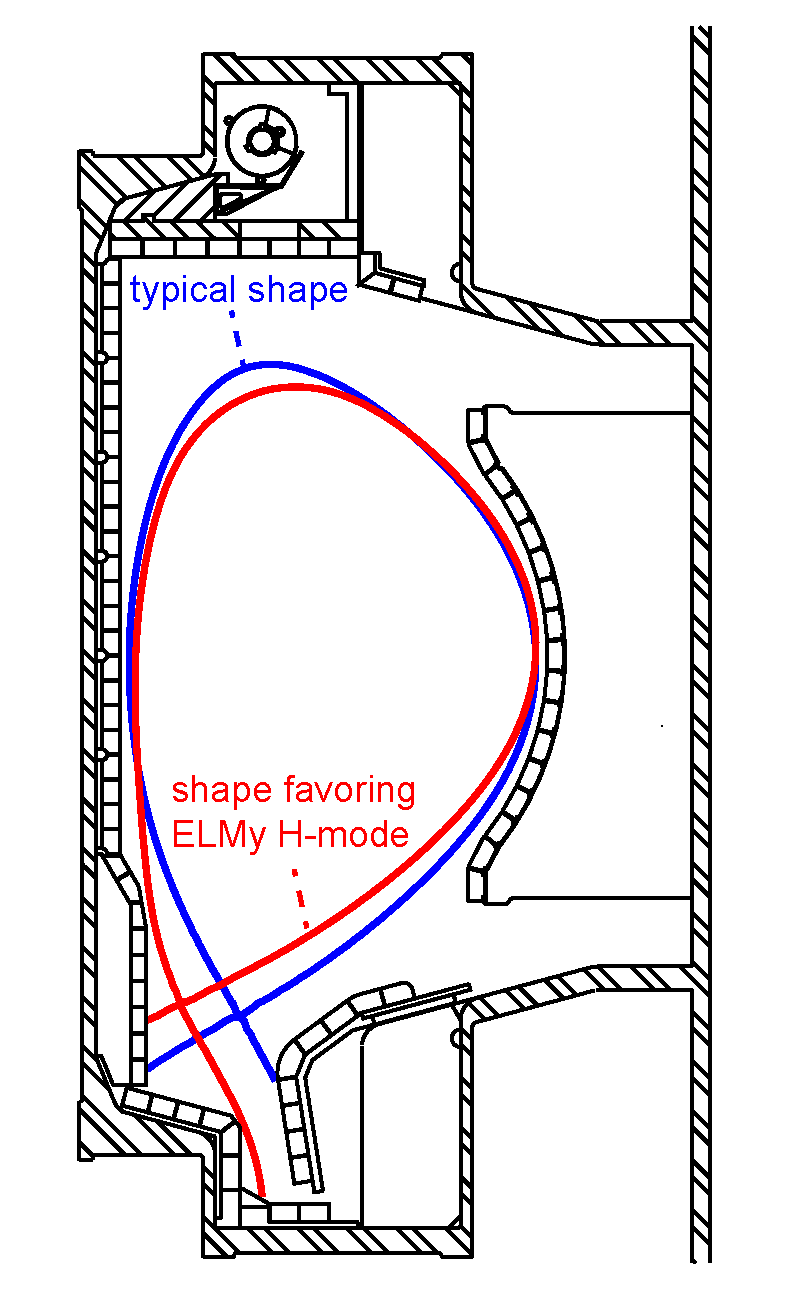
\includegraphics[width=90mm]{graphics/ELMy/shaping.pdf}}
\end{figure}

High-confinement operation on Alcator C-Mod differs is unique among major tokamak experiments in that typical H-modes do not exhibit the large Type-I ELMs\gnote{cite for this?} customarily seen on other devices.  Instead, ELM-free H-modes tend to form at lower collisionalities heating power levels, with high-density, high-power operation tending towards the continuously-regulated EDA H-mode rather than exhibiting discrete ELMs (see \cref{sec:hcr_elmfree,subsec:hcr_eda}).  However, by operating in a modified shape (see \cref{fig:elmy_shaping})\gnote{shape range} with low elongation and upper triangularity paired with high lower triangularity and a strike point on the divertor floor, regular ELMy H-mode operation is attainable.  This comparatively weak shaping, developed in similarity experiments with the JFT-2M tokamak \cite{Hughes2011}\gnote{better cite, Terry paper?}, reduces the necessary pressure gradient and bootstrap current to reach the ideal peeling-ballooning MHD stability boundary (described in \cref{sec:mod_pb}), triggering the ELM.  In this shape, new experiments on C-Mod \cite{Walk2012} attained ELMy H-modes across a broad range in current ($400-1100 \;\si{\kilo\ampere}$) and field ($3.5-8 \;\si{\tesla}$) with high-resolution pedestal data.

\begin{figure}[t]
 \pushtooutside
 \ffigbox[\FBwidth]{
\includegraphics[width=150mm]{graphics/ELMy/time_window.pdf}}{\caption{Example ELMy H-mode window (highlighted).  Phases for study are selected for steady density ($\overline{n}_e$ shown in the top trace), temperature (ECE $T_e$ signals shown for the core and pedestal), and ELM cycles ($D_\alpha$ signal shown).  The same modeling window is shown zoomed-in at the right.  Note the strong perturbation to the edge temperature due to the sawtooth crash.  Thomson scattering frames are indicated by the black ticks on the axes -- the ELM cycle is at a comparable frequency, $\sim \SI{60}{\hertz}$, to the TS system frame rate.  This presents a difficulty for selecting data masked to the ``peak'' of the ELM cycle, necessitating long, steady ELMing phases for study.}\label{fig:elmy_timewindow}}
\end{figure}

Pedestal profiles are taken with the edge Thomson scattering system, detailed in \cref{subsec:app_ts_cmod}.  The pedestal data is taken over steady ELMing phases to minimize the effects of random scatter in the data -- an example of such a window, with line-averaged density $\overline{n}_e$, core and edge $T_e$, and divertor $D_\alpha$ signal (indicative of the ELM crash), is shown in \cref{fig:elmy_timewindow}.  Strictly, models of the pedestal structure in ELMy H-mode predict the pedestal immediately preceding the ELM crash, when the pedestal is most unstable to the ELM trigger.  However, ELMs on C-Mod typically cycle at $60-100 \;\si{\hertz}$, comparable to the repetition rate of the Thomson scattering system (as shown in \cref{fig:elmy_timewindow}).  This presents difficulties in resolving the pedestal with multiple frames per ELM and binning the data to the peaks of the ELM cycle.  In most cases, pedestals are prepared in a single ``ensemble average'' utilizing all TS data in the window; in certain cases, a statistical set is also constructed using the last 20\% of the ELM cycle as is typical for other machines.  The results from this correction are discussed in \cref{sec:elmy_sync}.

\begin{figure}
 \pushtooutside
 \fcapside[65mm]{\caption{Example pedestal illustrating the $mtanh$ function used for pedestal fitting, defining the parameters: height $h$, baseline $b$, midpoint $x_0$, half-width $\delta$/full width $\Delta$.  The inboard slope is characterized by the parameter $\alpha$.}\label{fig:mtanh}}{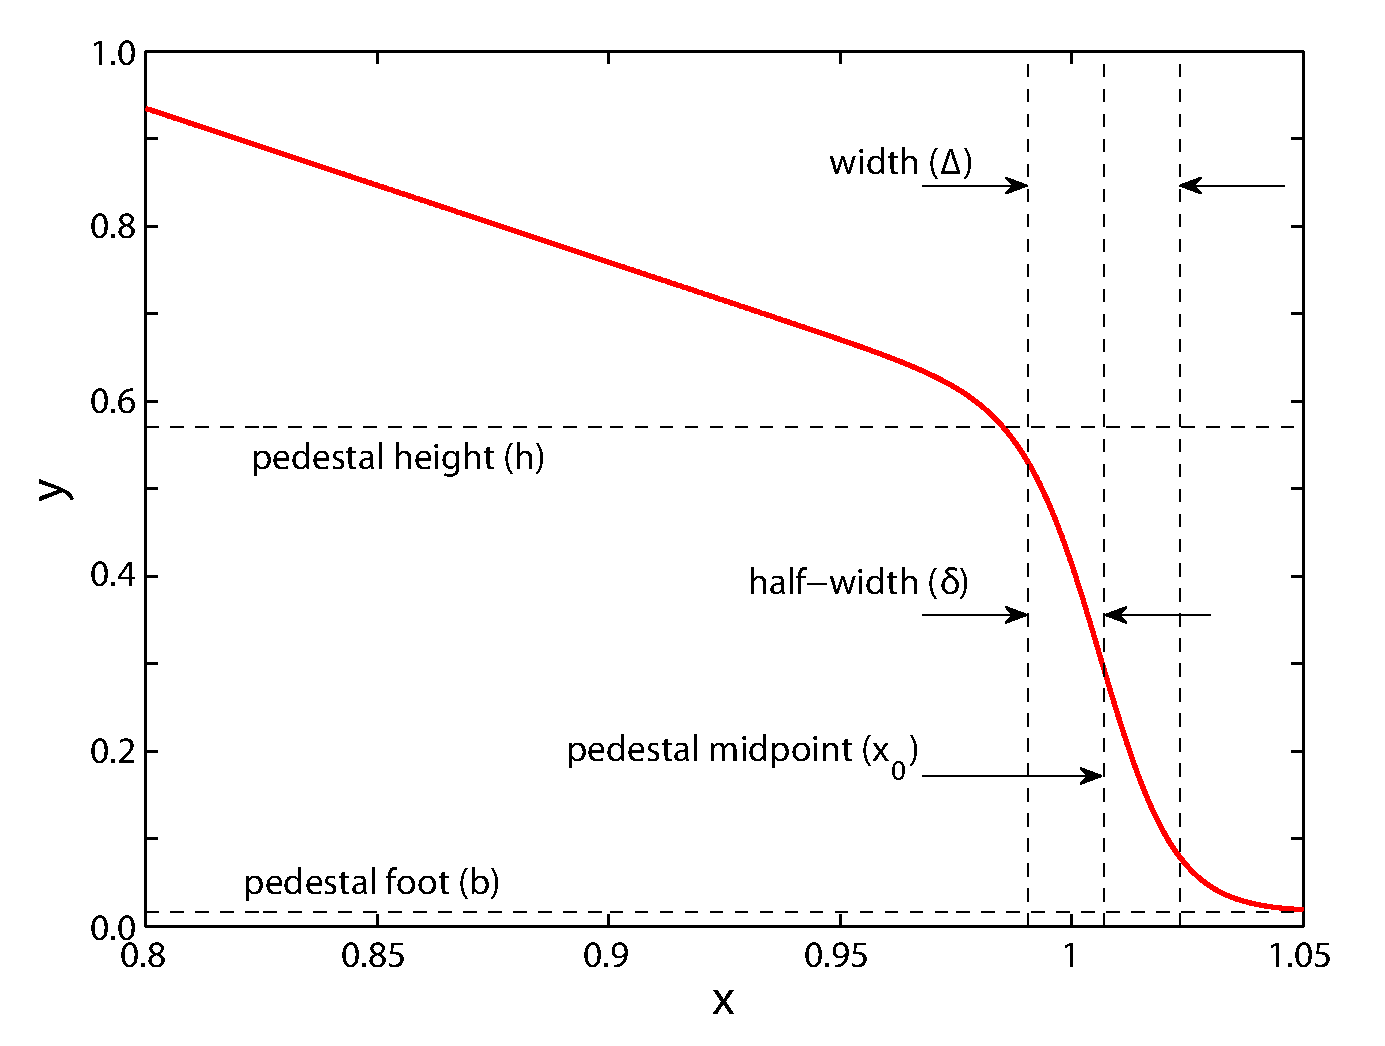
\includegraphics[width=100mm]{graphics/ELMy/mtanh.pdf}}
\end{figure}

The electron density, temperature, and pressure profiles are fitted using a modified hyperbolic-tangent fit developed in \cite{Groebner2001}.  In a general $x,y$ space, the fitting function is expressed by

\begin{equation}\label{eq:mtanh}
 \begin{aligned}
  z &= \frac{x_0 - x}{\delta}\\
  mtanh(\alpha,z) &= \frac{(1 + \alpha z) e^z - e^{-z}}{e^z + e^{-z}}\\
  y &= \frac{h+b}{2} + \frac{h-b}{2} mtanh(\alpha,z)
 \end{aligned}
\end{equation}

\noindent where $x_0$ is the pedestal midpoint, $h$ and $b$ are the height and baseline, and $\delta$ is the half-width (we use $\Delta = 2\delta$ as the ``pedestal width'').  The inboard slope is encoded by the parameter $\alpha$, with the multiplicative factor $1 + \alpha z$ providing a roughly linear profile far from the pedestal.  This definition provides a smooth, continuous definition for the pedestal gradient throughout the profile, with the peak gradient found analytically at $x_0$.\gnote{note similar $n_e$, $T_e$ pedestal widths, EPED width definition}

\nicesectionending

\section{ELM Cycle Synchronization}\label{sec:elmy_sync}

\nicesectionending

\section{EPED Model Predictions}\label{sec:elmy_eped}

\nicesectionending

\section{$I_p$ Scan}\label{sec:elmy_ip}

\nicesectionending

\section{Pedestal Width Scalings}\label{sec:elmy_width}

\nicechapterending

\bibliographystyle{../plainurl}
\bibliography{../references}